\chapter{Chân trời, phương trình trạng thái và năng lượng chân không}

\section{Hệ quy chiếu ưu tiên, sự lùi ra xa siêu quang và chân trời}

Phông vi sóng vũ trụ quả thật xác định một hệ quy chiếu đặc biệt. Trong hệ quy chiếu mà bức xạ đó trông đẳng hướng, các thiên hà lân cận cũng, xét trung bình, đứng yên. Nếu ta chuyển động qua phông này, các photon theo hướng phía trước sẽ bị dịch Doppler lên năng lượng cao hơn, còn các photon theo hướng phía sau sẽ bị dịch xuống năng lượng thấp hơn. Hệ quy chiếu ưu tiên là hệ trong đó phông vi sóng trông đẳng hướng, và đó cũng là, xét trung bình, hệ trong đó các thiên hà địa phương đứng yên.

\begin{classroomqa}
\lecturetimestamp{00:00:25}
\audiencequestion{Bước sóng biểu kiến của bức xạ vũ trụ có phụ thuộc vào chuyển động của người quan sát không, và điều đó có hàm ý một hệ quy chiếu ưu tiên không?}
\lecturerresponse{Có. Chuyển động qua phông vi sóng tạo ra tính dị hướng Doppler, nên tồn tại một hệ quy chiếu vũ trụ học ưu tiên: hệ trong đó phông vi sóng trông đẳng hướng. Đó cũng là, xét trung bình, hệ trong đó các thiên hà địa phương đứng yên.}
\end{classroomqa}

Một câu hỏi thứ hai liên quan đến các vận tốc lùi ra xa. Định luật Hubble nói rằng các thiên hà ở đủ xa tách xa nhau theo
\begin{equation}
v = H d .
\end{equation}
Với \(d\) đủ lớn, vận tốc lùi ra xa này vượt quá tốc độ ánh sáng. Điều đó không mâu thuẫn với thuyết tương đối, vì sự cấm đó chỉ có tính địa phương: một vật không thể đi vượt qua một vật khác ngay trước mặt chúng ta với tốc độ lớn hơn ánh sáng. Phát biểu về các thiên hà ở xa là một phát biểu về hình học giữa những nơi tách biệt rất xa nhau.

\begin{classroomqa}
\lecturetimestamp{00:04:48}
\audiencequestion{Hai thiên hà có thể có vận tốc tương đối lớn hơn \(c\) không?}
\lecturerresponse{Có, nếu chúng đủ xa nhau. Sự lùi ra xa theo Hubble có thể vượt quá tốc độ ánh sáng mà không vi phạm thuyết tương đối địa phương, và nơi mà vận tốc lùi ra xa đạt tới \(c\) là một chân trời.}
\end{classroomqa}

Một khi sự lùi ra xa đạt tới tốc độ ánh sáng, các tín hiệu gửi về phía chúng ta không còn tạo được sự tiến triển ròng nữa. Tia đó vẫn chuyển động, xét địa phương, với tốc độ giới hạn, nhưng quãng đường nó phải bù lại tăng quá nhanh.

\begin{classroomqa}
\lecturetimestamp{00:07:03}
\audiencequestion{Chẳng phải một tia sáng được gửi theo hướng ngược lại vẫn sẽ truyền về phía chúng ta sao?}
\lecturerresponse{Xét địa phương thì đúng, nhưng không gian giãn nở nhanh hơn mức tia đó có thể bù lại. Tia sáng chuyển động với tốc độ giới hạn so với các điểm lân cận, trong khi tổng khoảng cách trở về chỗ chúng ta vẫn tiếp tục tăng.}
\end{classroomqa}

\section{Metric giãn nở và phép loại suy với đường thẳng}

Một hình dung hữu ích là một chiều. Hãy tưởng tượng một đường thẳng được tạo thành từ các nguyên tử. Nếu ta kéo dãn một đường vật chất thông thường, cuối cùng nó sẽ đứt. Bây giờ hãy sửa đổi hình dung đó: mỗi khi các nguyên tử láng giềng tách nhau quá xa, ta chèn thêm một nguyên tử vào giữa chúng. Đường thẳng tiếp tục dài ra, nhưng tính chất địa phương của nó không bị thưa đi.

\begin{figure}
\centering
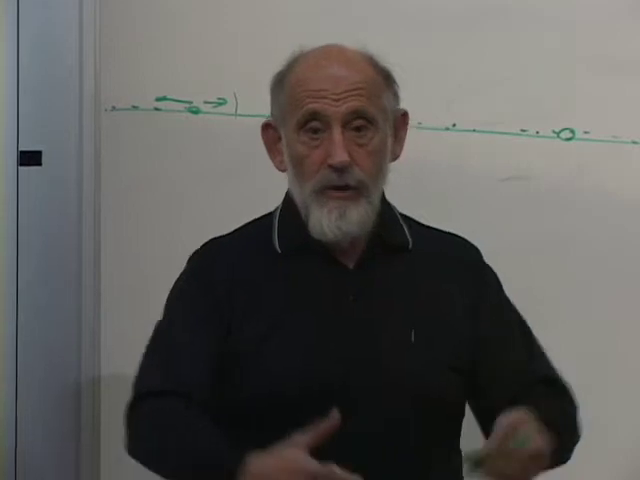
\includegraphics[width=0.60\textwidth]{lecture_04_figure_02.png}
\caption{Đường thẳng một chiều dùng để minh họa một metric giãn nở.}
\end{figure}

Trong hình dung này vẫn có một tốc độ tín hiệu giới hạn địa phương, cũng như âm thanh trên một đường thông thường có một tốc độ giới hạn. Quy tắc là địa phương: một nhiễu loạn không thể vượt quá tốc độ đó so với các điểm lân cận. Tuy vậy, nếu đường đủ dài và các điểm mới được chèn vào đủ nhanh, thì những phần đủ xa của nó lùi ra xa nhanh đến mức một tín hiệu sẽ không bao giờ có thể quay trở lại.

Vì thế, quy tắc cộng vận tốc của thuyết tương đối hẹp chỉ là một phần của vấn đề. Nó áp dụng ở mức địa phương, khi các người quan sát đi qua nhau tại cùng một điểm. Nó không phải là công cụ thích hợp cho các thiên hà cách xa nhau rất nhiều trong một hình học giãn nở.

\begin{classroomqa}
\lecturetimestamp{00:09:42}
\audiencequestion{Quy tắc tương đối tính thông thường để cộng vận tốc còn đúng trong tình huống này không?}
\lecturerresponse{Ở mức địa phương, tại một điểm, thì có. Nếu các người quan sát lần lượt đi qua nhau, quy tắc thông thường của thuyết tương đối hẹp áp dụng. Nhưng đó không phải là cách đúng để mô tả sự lùi ra xa nhanh hơn \(c\) giữa các thiên hà cách xa nhau rất nhiều; ở đó ta phải quay lại hình học của không gian giãn nở.}
\end{classroomqa}

Cùng hình dung đó cũng cho một cách giải thích đơn giản về độ dịch đỏ. Hãy vẽ một sóng trên đường thẳng. Khi đường thẳng giãn nở, bước sóng cũng giãn ra cùng nó. Trong một hình học giãn nở, đây không chỉ đơn thuần là một hình ảnh gợi ý. Các phương trình sóng trong không-thời gian giãn nở thật sự cho ra các bước sóng bị kéo dãn.

\begin{classroomqa}
\lecturetimestamp{00:14:42}
\audiencequestion{Phát biểu rằng một sóng bị kéo dãn cùng vũ trụ là mang tính lý thuyết, thực nghiệm, hay cả hai?}
\lecturerresponse{Đó là một hệ quả lý thuyết của sự truyền sóng trong không-thời gian giãn nở, và nó cũng được các quan sát thiên văn ủng hộ.}
\end{classroomqa}

Hình dung này không phải là một sợi dây cao su. Một sợi dây cao su sẽ mỏng đi khi bị kéo dãn, và một người sống trong một môi trường như vậy sẽ thấy các tính chất địa phương thay đổi. Ở đây các tính chất địa phương giữ nguyên, trong khi thang khoảng cách toàn cục tăng lên.

\section{Tán xạ cuối cùng và vũ trụ quan sát được}

Chân trời là nơi vận tốc lùi ra xa đạt tới tốc độ ánh sáng. Mặt tán xạ cuối cùng nằm hơi phía trong nó. Một tín hiệu phát ra từ chân trời sẽ bị kéo dãn vô hạn; bức xạ tán xạ cuối cùng có độ dịch đỏ rất lớn nhưng hữu hạn.

\begin{classroomqa}
\lecturetimestamp{00:17:53}
\audiencequestion{Mối quan hệ giữa sự lùi ra xa siêu quang, mặt tán xạ cuối cùng và vũ trụ quan sát được là gì?}
\lecturerresponse{Chân trời là nơi vận tốc lùi ra xa đạt tới tốc độ ánh sáng. Mặt tán xạ cuối cùng nằm hơi phía trong nó, vì độ dịch đỏ của nó là cực lớn nhưng hữu hạn. Về mặt thực tế, nó đánh dấu rìa của vũ trụ quan sát được.}
\end{classroomqa}

Độ dịch đỏ của bức xạ tán xạ cuối cùng xấp xỉ một hệ số \(10^3\). Mức đó đã lớn đến mức, đối với nhiều mục đích, mặt tán xạ cuối cùng rất gần chân trời. Vũ trụ quan sát được là phần của vũ trụ mà từ đó ánh sáng có thể tới được chúng ta.

Ở các thời điểm muộn, sự giãn nở tiến gần chế độ do năng lượng chân không chi phối. Khi đó đại lượng Hubble tiến tới một hằng số, chân trời tiến tới một kích thước cố định, và cả các thiên hà lẫn bức xạ vi sóng đều dần dần biến mất khỏi tầm nhìn.

\begin{classroomqa}
\lecturetimestamp{00:22:43}
\audiencequestion{Vì \(H\) thay đổi theo thời gian, khoảng cách tới chân trời có đang thay đổi không, và liệu cuối cùng phông vi sóng có biến mất không?}
\lecturerresponse{Ở các thời điểm muộn, \(H\) tiến tới một hằng số, nên chân trời tiến tới một khoảng cách cố định. Phông vi sóng tiếp tục bị kéo dãn, nguội đi và mờ dần. Các thiên hà ở xa cũng đi qua chân trời và biến mất khỏi tầm nhìn.}
\end{classroomqa}

Chỉ những cấu trúc vốn đã liên kết hấp dẫn mới còn nhìn thấy được. Hệ Mặt Trời không tách rời ra, và thiên hà cũng không tách rời ra, nhưng vũ trụ ở thang lớn trở thành một hòn đảo cô lập.

\section{Phương trình giãn nở cơ bản và ba thành phần}

Giờ đây phương trình giãn nở cơ bản là
\begin{equation}
\left(\frac{\dot a}{a}\right)^2 = \frac{8\pi G}{3}\rho ,
\qquad c=1 .
\end{equation}
Ở đây \(a(t)\) là thừa số tỉ lệ, còn \(\rho\) là mật độ năng lượng toàn phần.

\begin{figure}
\centering
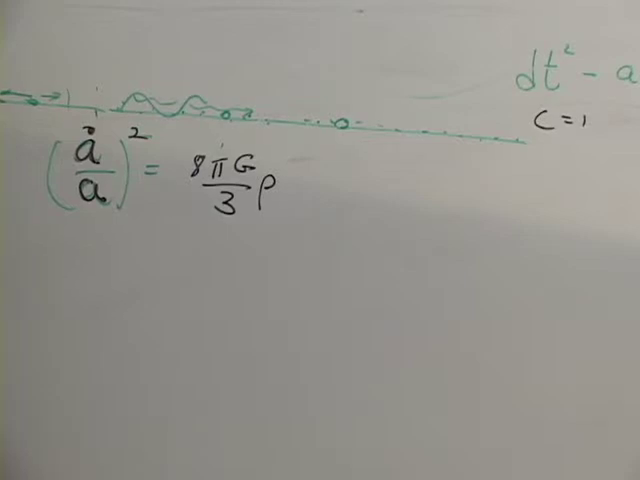
\includegraphics[width=0.74\textwidth]{lecture_04_figure_03.png}
\caption{Phương trình giãn nở cơ bản cùng với phép loại suy đường thẳng một chiều.}
\end{figure}

Có ba thành phần quan trọng về mặt động lực học.

Đối với vật chất,
\begin{equation}
\rho=\frac{\text{const.}}{a^3},
\qquad
a(t)\sim t^{2/3}.
\end{equation}
Đây là trường hợp của các vật có khối lượng chuyển động theo sự giãn nở tổng thể và về cơ bản đứng yên trong hệ quy chiếu đồng chuyển động.

Đối với bức xạ,
\begin{equation}
\rho=\frac{\text{const.}}{a^4},
\qquad
a(t)\sim t^{1/2}.
\end{equation}
Số mũ tăng thêm của \(a\) bắt nguồn từ sự dịch đỏ của từng photon khi vũ trụ giãn nở.

Cũng có
\begin{equation}
\rho_0=\text{constant},
\end{equation}
năng lượng chân không, còn được gọi là năng lượng tối hoặc, nếu bỏ qua các hệ số số học theo quy ước, là hằng số vũ trụ học. Thành phần này hoàn toàn không bị pha loãng.

Bước tiếp theo là liên hệ mật độ năng lượng với áp suất.

\section{Áp suất bức xạ và vật chất lạnh}

Hãy bắt đầu với bức xạ. Xét một hộp một chiều, chỉ là một đoạn thẳng có độ dài \(L\), chứa các photon bật qua bật lại. Trong một chiều, lực và áp suất về thực chất là cùng một thứ.

Xét một photon có độ lớn động lượng \(p\). Khi nó phản xạ từ một bức tường, động lượng của nó thay đổi một lượng
\begin{equation}
\Delta p = 2p.
\end{equation}
Khoảng thời gian giữa hai va chạm liên tiếp với cùng một bức tường là
\begin{equation}
\Delta t = \frac{2L}{c}.
\end{equation}
Vì vậy lực trung bình tác dụng lên bức tường là
\begin{equation}
F=\frac{\Delta p}{\Delta t}=\frac{pc}{L}.
\end{equation}
Đối với photon,
\begin{equation}
E=pc,
\end{equation}
nên
\begin{equation}
F=\frac{E}{L}.
\end{equation}
Năng lượng chia cho độ dài là mật độ năng lượng một chiều. Trong trường hợp một chiều này,
\begin{equation}
P=\rho .
\end{equation}

Với nhiều photon, sau khi lấy trung bình vẫn giữ nguyên quan hệ đó. Tổng lực đơn giản chính là tổng năng lượng trên một đơn vị độ dài.

Bây giờ hãy chuyển sang ba chiều. Nếu mọi photon chỉ chuyển động dọc theo một trục, chúng sẽ tác dụng áp suất lên một cặp mặt và không tác dụng gì lên các mặt kia. Điều đó cố ý là sai, nhưng nó cho thấy ngay điều gì cần được sửa. Trong một môi trường đẳng hướng, động lượng được phân bố theo mọi hướng. Trung bình, một phần ba mật độ năng lượng đóng góp vào mỗi thành phần áp suất. Kết quả là
\begin{equation}
P=\frac{\rho}{3}.
\end{equation}

Đối với vật chất lạnh thì câu trả lời khác. Hãy lấy một hộp đồng chuyển động, một vùng nhỏ chuyển động theo dòng chảy của vũ trụ. Các hạt bên trong mang năng lượng, nhưng nếu chúng đứng yên tương đối so với hộp thì chúng không đập vào các thành của nó. Vì vậy áp suất là
\begin{equation}
P=0.
\end{equation}

\begin{figure}
\centering
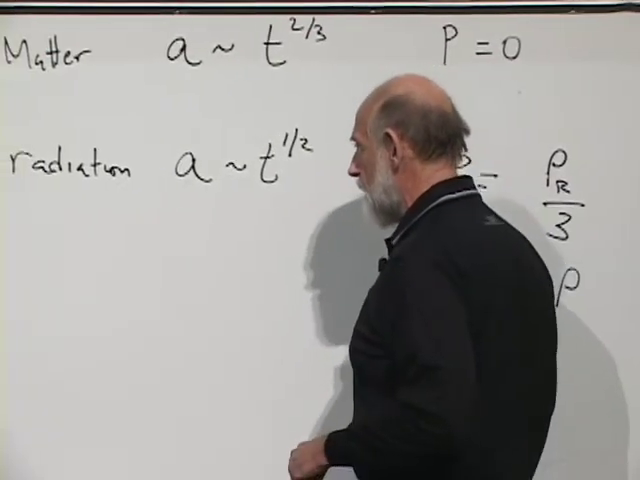
\includegraphics[width=0.74\textwidth]{lecture_04_figure_04.png}
\caption{Vật chất và bức xạ: \(a\sim t^{2/3}\), \(P=0\), và \(a\sim t^{1/2}\), \(P=\rho/3\).}
\end{figure}

Tóm tắt trên bảng là
\begin{align}
\text{matter:}\qquad & a(t)\sim t^{2/3}, \qquad P=0,\\
\text{radiation:}\qquad & a(t)\sim t^{1/2}, \qquad P=\frac{\rho}{3}.
\end{align}

\begin{classroomqa}
\lecturetimestamp{00:54:27}
\audiencequestion{Trong vũ trụ đang giãn nở, chẳng phải các hạt thực sự đang chuyển động tách xa nhau sao?}
\lecturerresponse{Có, nhưng lập luận về áp suất được áp dụng cho một hộp đồng chuyển động vô cùng nhỏ. Ở thang cục bộ đó, lập luận nhiệt động lực học vẫn còn đúng.}
\end{classroomqa}

\section{Phương trình trạng thái}

Áp suất được giả sử tỉ lệ với mật độ năng lượng,
\begin{equation}
P=w\rho .
\end{equation}
Trên bảng, cùng tham số đó được viết là \(\omega\). Đối với hai trường hợp cơ bản,
\begin{equation}
w=0 \quad \text{for cold matter},
\qquad
w=\frac{1}{3} \quad \text{for radiation}.
\end{equation}

Các trường hợp trung gian là có thể. Những giá trị giữa \(0\) và \(1/3\) mô tả vật chất không hoàn toàn lạnh cũng không hoàn toàn tương đối tính. Vật chất tối ấm là ví dụ được nhắc đến ở đây.

\begin{figure}
\centering
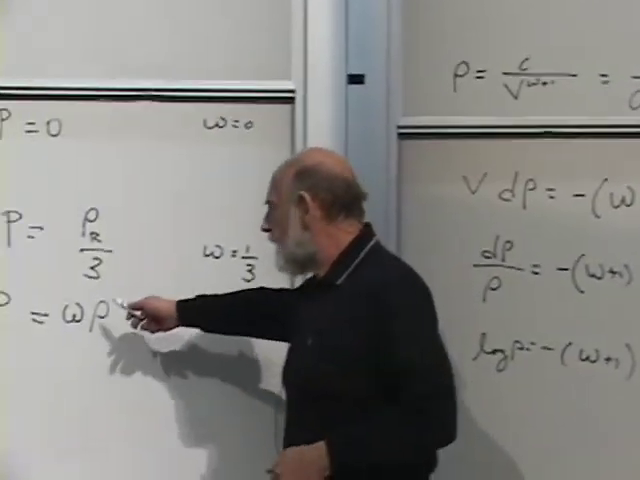
\includegraphics[width=0.74\textwidth]{lecture_04_figure_05.png}
\caption{Phương trình trạng thái \(P=\omega\rho\) cùng với lập luận về quy luật tỉ lệ của mật độ.}
\end{figure}

Câu hỏi tiếp theo là liệu \(w\) có chi phối sự phụ thuộc của \(\rho\) vào \(a\) hay không. Câu trả lời xuất phát từ một đồng nhất thức nhiệt động lực học.

Xét một hộp có thể tích \(V\). Nếu phần chứa trong đó gây áp suất \(P\), thì khi hộp giãn ra thêm \(dV\), công tác dụng lên các thành là
\begin{equation}
dE=-P\,dV.
\end{equation}
Bây giờ viết năng lượng dưới dạng
\begin{equation}
E=\rho V.
\end{equation}
Vi phân của nó là
\begin{equation}
dE=\rho\,dV+V\,d\rho .
\end{equation}
Đặt hai biểu thức bằng nhau, ta được
\begin{equation}
\rho\,dV+V\,d\rho=-P\,dV,
\end{equation}
hoặc
\begin{equation}
V\,d\rho=-(\rho+P)\,dV.
\end{equation}
Dùng \(P=w\rho\),
\begin{equation}
V\,d\rho=-(1+w)\rho\,dV.
\end{equation}
Chia cho \(\rho V\):
\begin{equation}
\frac{d\rho}{\rho}=-(1+w)\frac{dV}{V}.
\end{equation}
Lấy tích phân,
\begin{equation}
\rho \propto V^{-(1+w)}.
\end{equation}
Đối với một hộp vũ trụ học đồng chuyển động,
\begin{equation}
V\propto a^3,
\end{equation}
và do đó
\begin{equation}
\rho \propto a^{-3(1+w)}.
\end{equation}

Ta lập tức thu lại các trường hợp trước:
\begin{align}
w=0 &\Longrightarrow \rho \propto a^{-3},\\
w=\frac{1}{3} &\Longrightarrow \rho \propto a^{-4}.
\end{align}

Đó là lý do \(w\) quan trọng. Một khi đã biết \(\rho(a)\), ta có thể thế nó trở lại vào phương trình Friedmann. Khi đó ta thử một luật lũy thừa \(a\sim t^\alpha\) và xác định vũ trụ giãn nở như thế nào đối với phương trình trạng thái đó.

\section{Năng lượng chân không và áp suất âm}

Có một trường hợp đặc biệt có hành vi khác:
\begin{equation}
w=-1.
\end{equation}
Khi đó
\begin{equation}
1+w=0,
\end{equation}
nên số mũ triệt tiêu và
\begin{equation}
\rho=\rho_0=\text{constant}.
\end{equation}
Áp suất tương ứng là
\begin{equation}
P=-\rho .
\end{equation}

Áp suất âm tự nó không có gì bí ẩn. Áp suất dương đẩy ra ngoài lên các thành của một hộp. Áp suất âm kéo vào trong. Đó là lực căng. Một sợi dây cao su bị kéo dãn là ví dụ thường ngày: nó tích trữ năng lượng dương, nhưng kéo hai đầu của nó lại gần nhau.

Thế mật độ hằng \(\rho_0\) vào phương trình Friedmann:
\begin{equation}
\left(\frac{\dot a}{a}\right)^2=\frac{8\pi G}{3}\rho_0.
\end{equation}
Vế phải chỉ là một hằng số, nên
\begin{equation}
\frac{\dot a}{a}=\sqrt{\frac{8\pi G}{3}\rho_0}.
\end{equation}
Đây là trường hợp đặc biệt trong đó đại lượng Hubble thực sự là hằng số. Phương trình có thể viết thành
\begin{equation}
\dot a=\sqrt{\frac{8\pi G}{3}\rho_0}\,a,
\end{equation}
và nghiệm là
\begin{equation}
a(t)\propto \exp\!\left(\sqrt{\frac{8\pi G}{3}\rho_0}\,t\right).
\end{equation}

Đây là sự giãn nở theo hàm mũ. Thang thời gian thích hợp là thời gian tăng theo hệ số \(e\), không phải thời gian tăng gấp đôi, và ước lượng thô dùng ở đây đặt nó vào cỡ tuổi của vũ trụ. Năng lượng chân không và hằng số vũ trụ học là cùng một thành phần vật lý, khác nhau chỉ ở các quy ước số trị mang tính lịch sử.

\begin{classroomqa}
\lecturetimestamp{01:27:16}
\audiencequestion{Nếu năng lượng chân không gây ra sự giãn nở theo hàm mũ, chẳng phải cuối cùng mọi thứ sẽ bị xé rời sao?}
\lecturerresponse{Không nhất thiết. Các hệ liên kết có thể chống lại nó. Một thiên hà, một hệ Mặt Trời, hay một nguyên tử không nhất thiết bị xé rời, trong khi các cấu trúc đủ lớn và đủ loãng thì có tham gia vào sự giãn nở và cuối cùng tách rời nhau.}
\end{classroomqa}

\begin{classroomqa}
\lecturetimestamp{01:31:43}
\audiencequestion{Có điều gì đáng chú ý ở dấu âm khi lấy căn bậc hai của phương trình Friedmann không?}
\lecturerresponse{Có. Việc lấy căn bậc hai cho hai nhánh. Một nhánh là nghiệm giãn nở, và nhánh kia là nghiệm co lại khi đảo ngược thời gian. Bản thân các phương trình cho phép cả hai.}
\end{classroomqa}

\section{Ba thời kỳ và lịch sử giãn nở quan sát được}

Cả ba thành phần đều hiện diện, và chúng biến thiên theo các quy luật khác nhau:
\begin{equation}
\begin{aligned}
\rho_{\text{radiation}}&\propto a^{-4},\\
\rho_{\text{matter}}&\propto a^{-3},\\
\rho_0&=\text{constant}.
\end{aligned}
\end{equation}
Điều đó suy ra ngay ba thời kỳ.

Ở \(a\) rất nhỏ, bức xạ chi phối. Về sau, vật chất chi phối. Khi \(a\) đủ lớn, năng lượng chân không chi phối. Các quy luật giãn nở tương ứng là
\begin{equation}
a(t)\sim t^{1/2},
\qquad
a(t)\sim t^{2/3},
\qquad
a(t)\sim e^{Ht}.
\end{equation}

Những thời điểm xấp xỉ được nêu ở đây là như sau: bức xạ nhường chỗ cho vật chất sau khoảng \(10^4\) năm. Vũ trụ trở nên trong suốt muộn hơn, sau khoảng \(10^5\) năm. Sự chuyển tiếp từ giai đoạn vật chất chi phối sang giãn nở gia tốc xảy ra muộn hơn rất nhiều, sau vài tỷ năm, xấp xỉ vào giữa lịch sử vũ trụ theo ước lượng bậc độ lớn đang được dùng.

Lịch sử này được suy ra như thế nào? Chúng ta không thể thấy tương lai, nhưng có thể thấy quá khứ. Nhìn ra khoảng cách lớn hơn nghĩa là nhìn về thời điểm sớm hơn. Bằng cách quan sát các thiên hà xa, đo cách chuyển động của chúng tương quan với khoảng cách, và tái dựng đại lượng Hubble như một hàm của thời gian nhìn ngược, người ta tái dựng được lịch sử theo thời gian của thừa số tỉ lệ. Thời kỳ bức xạ chi phối diễn ra quá sớm nên không thể thấy trực tiếp trong thiên văn học thiên hà thông thường, nhưng thời kỳ vật chất chi phối và sự chuyển tiếp sang giai đoạn chân không chi phối thì hiện rõ trên đường cong được tái dựng.

\section{Tán xạ cuối cùng trong tương lai xa}

Bầu trời vi sóng trong tương lai không phải cùng một hiện tượng như việc các thiên hà biến mất qua chân trời. Bức xạ mà ta thấy ở những thời điểm muộn hơn đến từ vật chất ở xa hơn, nên hiệu ứng là nhìn ngày càng sâu hơn và lạnh hơn chứ không phải chứng kiến chính những nguyên tử ấy đơn giản lùi xa đi.

\begin{classroomqa}
\lecturetimestamp{01:48:07}
\audiencequestion{Nếu mặt tán xạ cuối cùng mờ dần vào chân trời, điều đó có phải cũng chính là chuyện các thiên hà đi ra ngoài chân trời không?}
\lecturerresponse{Không. Bức xạ về sau không đến từ cùng những nguyên tử như bức xạ ta thấy bây giờ. Nó đến từ những nguyên tử ở xa hơn, nên giống như nhìn ngày càng sâu hơn vào vũ trụ, trong khi bức xạ trông ngày càng lạnh hơn.}
\end{classroomqa}

\section{Độ cong, bức tranh Big Crunch, và chân trời ở thời muộn}

Cho đến đây, số hạng độ cong đã được lược bỏ. Khôi phục nó ta được
\begin{equation}
\left(\frac{\dot a}{a}\right)^2
=
\frac{8\pi G}{3}\rho
-
\frac{K}{a^2}.
\end{equation}
Về mặt số trị, số hạng này có vẻ nhỏ, nhưng về mặt khái niệm nó quan trọng. Trong ngôn ngữ Newton cổ hơn, nó phân biệt các trường hợp tổng năng lượng dương, bằng không và âm. Trong ngôn ngữ tương đối tính, nó phân biệt các hình học không gian.

Trước khi năng lượng chân không được xem xét nghiêm túc, người ta thường hình dung một vũ trụ bị vật chất chi phối trong đó sự giãn nở rốt cuộc sẽ đảo chiều. Kết quả là bức tranh Big-Crunch cũ: giãn nở từ Big Bang, rồi co trở lại. Toán học vẫn còn đúng, nhưng dường như nó không còn mô tả vũ trụ của chúng ta nữa.

\begin{classroomqa}
\lecturetimestamp{01:53:51}
\audiencequestion{Năng lượng chân không này có liên quan đến năng lượng chân không lượng tử không?}
\lecturerresponse{Có, hoặc ít nhất người ta tin là như vậy.}
\end{classroomqa}

Thành phần xấp xỉ của vũ trụ ngày nay là
\begin{equation}
\frac{\rho_0}{\rho_{\text{total}}}\sim 0.7,
\qquad
\frac{\rho_{\text{matter}}}{\rho_{\text{total}}}\sim 0.3.
\end{equation}
Trong thành phần vật chất đó, vật chất phát sáng chiếm khoảng \(0.05\) và vật chất tối chiếm khoảng \(0.25\) của toàn bộ. Ngày nay, bức xạ là không đáng kể. Vật chất tối và vật chất phát sáng biến thiên cùng một cách, nên tỉ số của chúng giữ nguyên ngay cả khi độ phong phú tương đối của vật chất, bức xạ và chân không thay đổi từ thời kỳ này sang thời kỳ khác.

Trong giới hạn chân không chi phối,
\begin{equation}
H=\sqrt{\frac{8\pi G}{3}\rho_0}.
\end{equation}
Khi đó định luật Hubble trở thành
\begin{equation}
v=Hd.
\end{equation}
Chân trời được xác định bởi \(v=1\), nên khoảng cách của nó là
\begin{equation}
d_H=\frac{1}{H}
=
\frac{1}{\sqrt{8\pi G\rho_0/3}}.
\end{equation}
Con số xấp xỉ được nêu ở đây là khoảng \(10\) đến \(12\) tỷ năm ánh sáng.

Điểm quan trọng là hành vi ở thời muộn. Một khi sự giãn nở là theo hàm mũ, khoảng cách chân trời trở nên cố định. Các thiên hà tiếp tục đi qua nó và biến mất do bị dịch đỏ ngày càng mạnh. Phông vi sóng cũng bị dịch đỏ đến mức biến mất. Trong tương lai rất xa, chỉ còn những cấu trúc ở gần bị liên kết hấp dẫn là còn quan sát được, và vũ trụ trông như một hòn đảo cô lập.

\section{Hình học từ mặt tán xạ cuối cùng}

Cuối cùng, hình học có thể được kiểm định từ bề mặt tán xạ cuối cùng. Giả sử khoảng cách đến bề mặt đó đã biết. Cũng giả sử rằng người ta có thể nhận diện ở đó một đốm mà kích thước vật lý của nó được biết đủ chính xác. Khi đó có thể so sánh kích thước ấy và khoảng cách ấy với kích thước góc quan sát được.

Trong không gian phẳng, góc là góc Euclid. Trong không gian cong dương, nó sẽ có vẻ lớn hơn; trong không gian cong âm, nhỏ hơn. Phép loại suy ở đây là phép trắc đạc thông thường: lấy một vật có kích thước đã biết ở một khoảng cách đã biết rồi so sánh góc đo được với hình học Euclid.

\begin{classroomqa}
\lecturetimestamp{02:08:09}
\audiencequestion{Một ví dụ về một vật ở đó mà ta biết kích thước của nó là gì?}
\lecturerresponse{Những đốm lớn nhất trong phông vi sóng. Chúng ta nghĩ rằng mình biết kích thước của chúng từ thời gian chúng mất để tiến hóa và từ tốc độ âm thanh.}
\end{classroomqa}

Các vật thể liên quan ở đây là những đốm lớn nhất trên phông vi sóng. Kích thước góc quan sát được của chúng cho kết quả phù hợp với hình học Euclid trong phạm vi vài phần trăm. Trên cơ sở đó, không gian có vẻ phẳng.

\section{Giá trị đo được của \(w\) và một câu hỏi cuối cùng}

Tầm quan trọng về mặt quan sát của \(w\) giờ đây đã rõ. Nếu các nhà thiên văn báo cáo rằng \(w\) rất gần \(-1\), thì họ đang nói rằng thành phần năng lượng chân không gần như là hằng. Đó chính là ý được nêu ở đây.

Điều đó không có nghĩa là thuyết tương đối rộng buộc \(w\) phải đúng bằng \(-1\). Vấn đề ở đây là thực nghiệm. Bài giảng có ghi chú ngắn gọn rằng về nguyên tắc, những khả năng triệt để hơn không bị loại trừ, nhưng trường hợp năng lượng chân không gần như hằng là trường hợp mà ta có cơ sở vững để tin.

\begin{classroomqa}
\lecturetimestamp{02:11:04}
\audiencequestion{Trong việc tính mật độ của vật chất và của bức xạ, có phải chúng ta đã giả sử năng lượng là không đổi rồi sau đó điều chỉnh thừa số tỉ lệ để suy ra công thức không? Và nếu điều đó đúng cho hai trường hợp đầu, thì trong trường hợp năng lượng chân không, ở đó mật độ vẫn không đổi, điều gì xảy ra?}
\lecturerresponse{Không. Tôi không giả sử nó là không đổi. Chúng ta đã dùng hệ thức rằng độ biến thiên năng lượng bằng \(-P\,dV\). Đối với một hộp đồng chuyển động tưởng tượng đi cùng với sự giãn nở, có công tác dụng lên các thành hộp, và điều đó giải thích cho sự thay đổi năng lượng. Trường hợp năng lượng chân không đặt ra câu hỏi theo một cách khác, và nhận xét kết lại ở đây là cách nói về bảo toàn năng lượng trong vũ trụ học không cho biết được bao nhiêu, vì tổng năng lượng của vũ trụ bằng không.}
\end{classroomqa}
